%!TEX program = xelatex
\documentclass[11pt]{beamer}

\usepackage{amsfonts}
\usepackage{amsmath}
\usepackage{blindtext}
\usepackage{enumitem}
\usepackage{fancyvrb}
\usepackage{tikz}

\usetheme{SaoPaulo}

\title{Numerical Python}
\subtitle{modeling, state}
\author{CS101 Lecture \#16}
\date{2016-11-23}

\setcounter{showSlideNumbers}{1}

\newcommand{\correctstar}{\textcolor{red}{$\star$}}

\begin{document}
  \setcounter{showProgressBar}{0}
  \setcounter{showSlideNumbers}{0}

%%%%%%%%%%%%%%%%%%%%%%%%%%%%%%%%%%%%%%%%%%%%%%%%%%%%%%%%%%%%%%%%%%%%%%%%%%%%%%%%
\frame{\titlepage}

%%%%%%%%%%%%%%%%%%%%%%%%%%%%%%%%%%%%%%%%%%%%%%%%%%%%%%%%%%%%%%%%%%%%%%%%%%%%%%%%
\setcounter{framenumber}{0}
\setcounter{showProgressBar}{1}
\setcounter{showSlideNumbers}{1}

%%%%%%%%%%%%%%%%%%%%%%%%%%%%%%%%%%%%%%%%%%%%%%%%%%%%%%%%%%%%%%%%%%%%%%%%%%%%%%%%
\section{Administrivia}

%%%%%%%%%%%%%%%%%%%%%%%%%%%%%%%%%%%%%%%%%%%%%%%%%%%%%%%%%%%%%%%%%%%%%%%%%%%%%%%%
\begin{frame}
  \frametitle{Administrivia}
  \Enlarge

  \begin{itemize}
  \myitem  Homework \#7 is due Friday, Nov.\ 25.
  \myitem  Homework \#8 is due Friday, Dec.\ 2.
  \end{itemize}
\end{frame}


%%%%%%%%%%%%%%%%%%%%%%%%%%%%%%%%%%%%%%%%%%%%%%%%%%%%%%%%%%%%%%%%%%%%%%%%%%%%%%%%
\section{More \texttt{numpy}}

%%%%%%%%%%%%%%%%%%%%%%%%%%%%%%%%%%%%%%%%%%%%%%%%%%%%%%%%%%%%%%%%%%%%%%%%%%%%%%%%
\begin{frame}[fragile]
  \frametitle{Indexing arrays}
  \Enlarge

  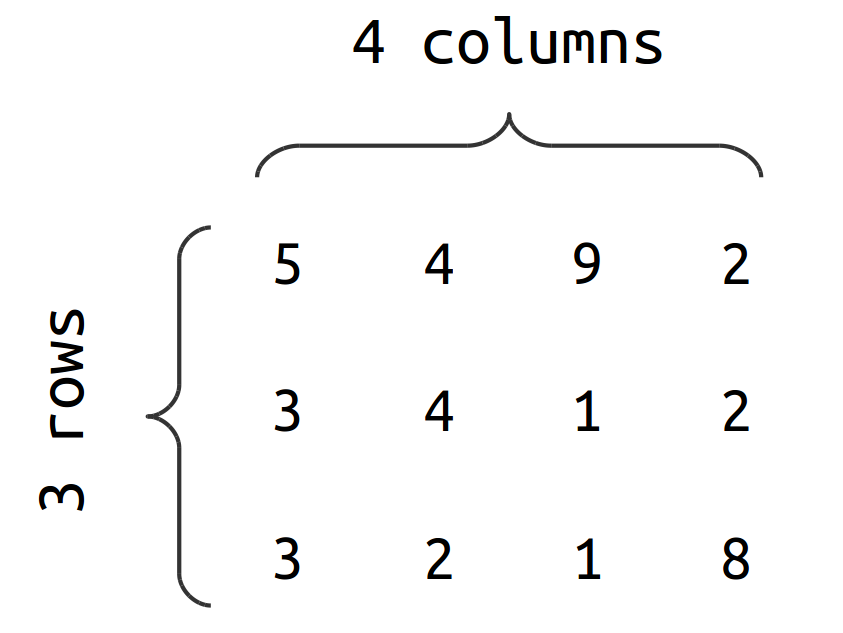
\includegraphics[width=0.67\textwidth]{./img/ndarray.png}

  \begin{enumerate}
  \myitem  Reminder:  \texttt{numpy} indexes by \texttt{array[row][col]}.
  \end{enumerate}
\end{frame}

%%%%%%%%%%%%%%%%%%%%%%%%%%%%%%%%%%%%%%%%%%%%%%%%%%%%%%%%%%%%%%%%%%%%%%%%%%%%%%%%
\begin{frame}[fragile]
  \frametitle{Question}
  \Enlarge

$$
x =
\left(
\begin{array}{cc}
1 & 1 \\
2 & 2 \\
3 & 3
\end{array}
\right)
$$

  What will produce this array?

  \begin{enumerate}[label=\Alph*]
  \item
  \begin{Verbatim}
np.array([[1,2,3],[1,2,3]])
  \end{Verbatim}
  \item
  \begin{Verbatim}
np.array([2,3])
  \end{Verbatim}
  \item
  \begin{Verbatim}
np.array([3,2])
  \end{Verbatim}
  \item
  \begin{Verbatim}
np.array([[1,1],[2,2],[3,3]])
  \end{Verbatim}
  \end{enumerate}
\end{frame}

%%%%%%%%%%%%%%%%%%%%%%%%%%%%%%%%%%%%%%%%%%%%%%%%%%%%%%%%%%%%%%%%%%%%%%%%%%%%%%%%
\begin{frame}[fragile]
  \frametitle{Question}
  \Enlarge

$$
x =
\left(
\begin{array}{cc}
1 & 1 \\
2 & 2 \\
3 & 3
\end{array}
\right)
$$

  What will produce this array?

  \begin{enumerate}[label=\Alph*]
  \item
  \begin{Verbatim}
np.array([[1,2,3],[1,2,3]])
  \end{Verbatim}
  \item
  \begin{Verbatim}
np.array([2,3])
  \end{Verbatim}
  \item
  \begin{Verbatim}
np.array([3,2])
  \end{Verbatim}
  \item
  \begin{Verbatim}
np.array([[1,1],[2,2],[3,3]])
  \end{Verbatim}
  \correctstar
  \end{enumerate}
\end{frame}

%%%%%%%%%%%%%%%%%%%%%%%%%%%%%%%%%%%%%%%%%%%%%%%%%%%%%%%%%%%%%%%%%%%%%%%%%%%%%%%%
\begin{frame}[fragile]
  \frametitle{Data types}
  \Enlarge

  \begin{enumerate}
  \myitem  \texttt{numpy} supports many possible data types:
    \begin{enumerate}
    \mysubitem  \texttt{bool}
    \mysubitem  \texttt{int16}, \texttt{int32}
    \mysubitem  \texttt{float16}, \texttt{float32}, \texttt{float64}
    \mysubitem  \texttt{complex64}, \texttt{complex128}
    \end{enumerate} %\pause
  \myitem  For the most part, stick with \texttt{bool}, \texttt{int32}, and \texttt{float64} (most accurate).
  \myitem  Specify (and query) with \texttt{dtype}:
  \end{enumerate}
  \begin{Verbatim}
import numpy as np
a = [ 3,2,4 ]
x = np.array( a,dtype=np.float64 )
x.dtype
  \end{Verbatim}
\end{frame}

%%%%%%%%%%%%%%%%%%%%%%%%%%%%%%%%%%%%%%%%%%%%%%%%%%%%%%%%%%%%%%%%%%%%%%%%%%%%%%%%
\begin{frame}[fragile]
  \frametitle{Other arrays}
  \Enlarge

  \begin{Verbatim}
x = np.zeros( [ 2,3 ] ) # zeroes
y = np.ones( [ 4,1 ] )  # ones
  \end{Verbatim}
  \begin{enumerate}
  \myitem  Produce arrays of zeros or ones with specified dimensions.
  \end{enumerate}
\end{frame}

%%%%%%%%%%%%%%%%%%%%%%%%%%%%%%%%%%%%%%%%%%%%%%%%%%%%%%%%%%%%%%%%%%%%%%%%%%%%%%%%
\begin{frame}[fragile]
  \frametitle{Other arrays}
  \Enlarge

  \begin{Verbatim}
z = np.eye( 5 )         # identity
  \end{Verbatim}
  \begin{enumerate}
  \myitem  Produces identity matrix of specified square dimension.
  \end{enumerate}
\end{frame}

%%%%%%%%%%%%%%%%%%%%%%%%%%%%%%%%%%%%%%%%%%%%%%%%%%%%%%%%%%%%%%%%%%%%%%%%%%%%%%%%
\begin{frame}[fragile]
  \frametitle{Other arrays}
  \Enlarge

  \begin{Verbatim}
w = np.linspace( 0,10,101 )
v = np.linspace( start, finish, n)
  \end{Verbatim}
  \begin{enumerate}
  \myitem  Produce arrays from \texttt{start} to \texttt{finish} of \texttt{n} points (\emph{not} spacing!).
  \myitem  Excellent for grids and coordinates.
  \myitem  May also see \texttt{arange}: [start, stop), but I recommend avoiding its use:
  \end{enumerate}
  \begin{Verbatim}
u = np.arange( 0,10,0.1 )  # tricky!
u == array( [ 0, 0.1, 0.2, ..., 9.9 ] )
  \end{Verbatim}
\end{frame}

%%%%%%%%%%%%%%%%%%%%%%%%%%%%%%%%%%%%%%%%%%%%%%%%%%%%%%%%%%%%%%%%%%%%%%%%%%%%%%%%
\begin{frame}[fragile]
  \frametitle{The punchline:  Why?}
 % \Enlarge

  Plot $sin(x)$ for $x \in \left[ 0, 2\pi \right]$ using pure Python.
  %\pause

  \begin{Verbatim}
import matplotlib.pyplot as plt
%matplotlib inline  
from math import pi
x = []   # can't use range!
for i in range(100):
    x.append( 2*pi*i/100 )
from math import sin
y = []
for j in range(100):
    y.append( sin(x[j]) )
plt.plot( x,y,'k-' )
plt.xlim( 0,2*pi )
plt.ylim( -1,1 )
plt.show()
  \end{Verbatim}
  
\end{frame}

%%%%%%%%%%%%%%%%%%%%%%%%%%%%%%%%%%%%%%%%%%%%%%%%%%%%%%%%%%%%%%%%%%%%%%%%%%%%%%%%
\begin{frame}[fragile]
  \frametitle{The punchline:  Why?}
  \Enlarge

  Plot $sin(x)$ for $x \in \left[ 0, 2\pi \right]$ using \texttt{numpy}.
  %\pause

  \begin{Verbatim}
import matplotlib.pyplot as plt
%matplotlib inline  
import numpy as np
x = np.linspace( 0,2*np.pi,101 )
y = np.sin( x )

plt.plot( x,y,'k-' )
plt.xlim( 0,2*pi )
plt.ylim( -1,1 )
plt.show()
  \end{Verbatim}
  
 See options for plot at \url{http://stackoverflow.com/questions/8376926/plotting-many-graphs-with-matplotlib}
 
\end{frame}

% Lecture16 slides 37--63

%%%%%%%%%%%%%%%%%%%%%%%%%%%%%%%%%%%%%%%%%%%%%%%%%%%%%%%%%%%%%%%%%%%%%%%%%%%%%%%%
\section{Modeling}

%%%%%%%%%%%%%%%%%%%%%%%%%%%%%%%%%%%%%%%%%%%%%%%%%%%%%%%%%%%%%%%%%%%%%%%%%%%%%%%%
\begin{frame}[fragile]
  \frametitle{Modeling}
  \Enlarge

  Consider a cup falling from the edge of a table.  Describe its path and time until it hits the ground. %\pause

  Two approaches:
  \begin{enumerate}
  \myitem  Use analytical equation (if available).
  \myitem  Use finite difference equation otherwise.
  \end{enumerate}
\end{frame}

%%%%%%%%%%%%%%%%%%%%%%%%%%%%%%%%%%%%%%%%%%%%%%%%%%%%%%%%%%%%%%%%%%%%%%%%%%%%%%%%
\begin{frame}[fragile]
  \frametitle{Modeling}
  \Enlarge

  \begin{enumerate}
  \myitem  Use analytical equation (if available).
  \end{enumerate}

$$
y(t) = y_0 + v_0 t + \frac{a}{2} t^{2}
$$
$$
y_0 = 1
$$
$$
v_0 = 0
$$
$$
a = -9.8
$$
subject to
$$
y(t) \geq 0
$$
\end{frame}

%%%%%%%%%%%%%%%%%%%%%%%%%%%%%%%%%%%%%%%%%%%%%%%%%%%%%%%%%%%%%%%%%%%%%%%%%%%%%%%%
\begin{frame}[fragile]
  \frametitle{Modeling}

  \begin{Verbatim}
import numpy as np

# Parameters of simulation
n = 100     # number of data points to plot
start = 0.0 # start time, s
end = 1.0   # ending time, s
a = -9.8    # acceleration, m*s**-2

# State variable initialization
t = np.linspace(start,end,n+1) # time, s

y = 1.0 + a/2 * t**2

for i in range(1,n+1):
    if y[i] <= 0: # glass has hit the ground
        y[i] = 0
  \end{Verbatim}
\end{frame}

%%%%%%%%%%%%%%%%%%%%%%%%%%%%%%%%%%%%%%%%%%%%%%%%%%%%%%%%%%%%%%%%%%%%%%%%%%%%%%%%
\begin{frame}[fragile]
  \frametitle{Modeling}
  \Enlarge

  \begin{enumerate}
  \myitem  Use finite difference equation otherwise.
  \end{enumerate}

$$
\frac{dy}{dt} = v(t) \approx \frac{y^{n+1} - y^{n}}{t^{n+1} - t^{n}} \rightarrow y^{n+1} = y^{n} + v \left( t^{n+1} - t^{n} \right)
$$
$$
\frac{dv}{dt} = a \approx \frac{v^{n+1} - v^{n}}{t^{n+1} - t^{n}} \rightarrow v^{n+1} = v^{n} + a \left( t^{n+1} - t^{n} \right)
$$
$$
v^{n=0} = 0
\hspace{2cm}
y^{n=0} = 1
\hspace{2cm}
a = -9.8
$$
subject to
$$
y(t) \geq 0
$$
\end{frame}

%%%%%%%%%%%%%%%%%%%%%%%%%%%%%%%%%%%%%%%%%%%%%%%%%%%%%%%%%%%%%%%%%%%%%%%%%%%%%%%%
\begin{frame}[fragile]
  \frametitle{Modeling}
  \Enlarge

  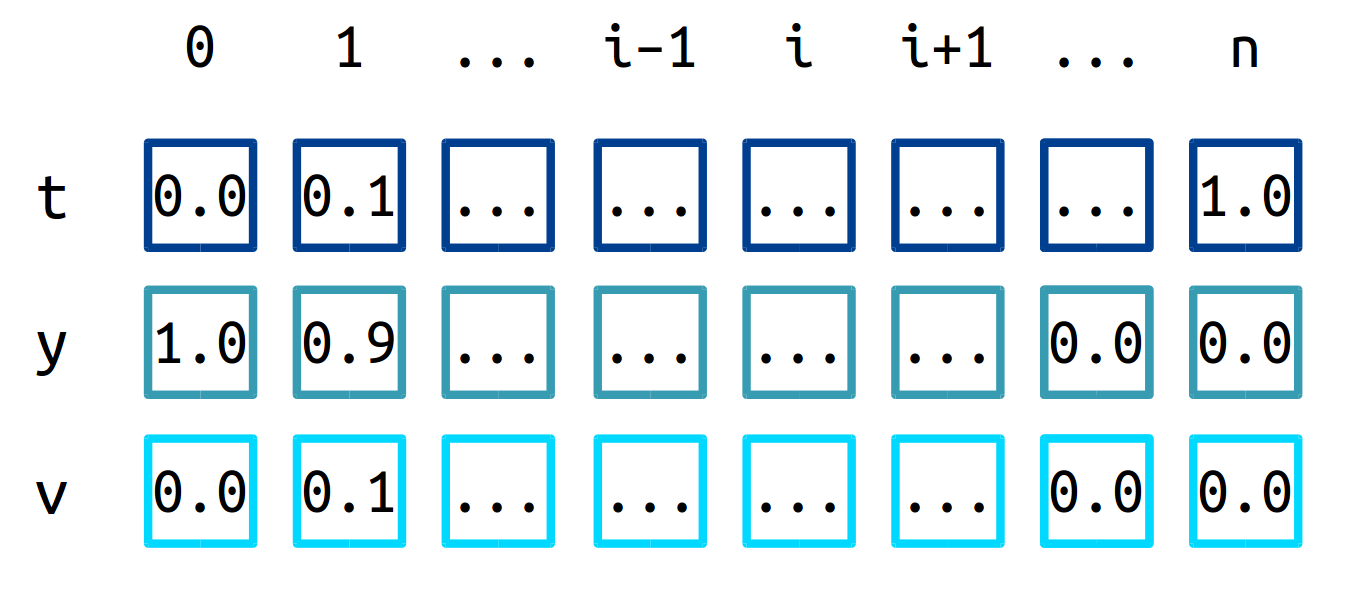
\includegraphics[width=0.8\textwidth]{./img/arrays.png}
\end{frame}

%%%%%%%%%%%%%%%%%%%%%%%%%%%%%%%%%%%%%%%%%%%%%%%%%%%%%%%%%%%%%%%%%%%%%%%%%%%%%%%%
\begingroup
\footnotesize
\begin{frame}[fragile]
  \frametitle{Modeling}

  \begin{Verbatim}

import numpy as np

# Parameters of simulation
n = 100     # number of data points to plot
start = 0.0 # start time, s
end = 1.0   # ending time, s
a = -9.8    # acceleration, m*s**-2

# State variable initialization
t = np.linspace(start,end,n+1) # time, s
y = np.zeros(n+1)              # height, m
v = np.zeros(n+1)              # velocity, m*s**-1
y[0] = 1.0                     # initial condition, m

for i in range(1,n+1):
    v[i] = v[i-1] + a*( t[i]-t[i-1] )
    y[i] = y[i-1] + v[i-1] * ( t[i]-t[i-1] )

    if y[i] <= 0: # glass has hit the ground
        v[i] = 0
        y[i] = 0
  \end{Verbatim}
\end{frame}
\endgroup

%%%%%%%%%%%%%%%%%%%%%%%%%%%%%%%%%%%%%%%%%%%%%%%%%%%%%%%%%%%%%%%%%%%%%%%%%%%%%%%%
\begin{frame}[fragile]
  \frametitle{Modeling}
  \Enlarge

  \begin{enumerate}
  \myitem  How would you make the cup bounce? %\pause (Reverse the direction at the ground; have a decay factor.) %\pause
  \myitem  How would you include lateral motion? %\pause (Have separate $x$- and $y$-positions and velocities.)
  \end{enumerate}
\end{frame}

%%%%%%%%%%%%%%%%%%%%%%%%%%%%%%%%%%%%%%%%%%%%%%%%%%%%%%%%%%%%%%%%%%%%%%%%%%%%%%%%
\section{Reminders}

%%%%%%%%%%%%%%%%%%%%%%%%%%%%%%%%%%%%%%%%%%%%%%%%%%%%%%%%%%%%%%%%%%%%%%%%%%%%%%%%
\begin{frame}
  \frametitle{Reminders}
  \Enlarge

  \begin{itemize}
  \myitem  Homework \#7 is due Friday, Nov.\ 25.
  \myitem  Homework \#8 is due Friday, Dec.\ 2.
  \end{itemize}
\end{frame}

\end{document}
